\documentclass[DIN, pagenumber=false, fontsize=11pt, parskip=half]{scrartcl}

\usepackage{amsmath}
\usepackage{amsfonts}
\usepackage{amssymb}
\usepackage{enumitem}
\usepackage[utf8]{inputenc} 
\usepackage[ngerman]{babel} 
\usepackage[T1]{fontenc} 
\usepackage{pgfplots}
\usepackage{xcolor}
\usepackage{listings}
\usepackage{float}
\usepackage{graphicx}
\usepackage{booktabs}
\usepackage{tkz-euclide}
\usepackage{svg}
\usepackage{trfsigns}

\definecolor{mygreen}{RGB}{28,172,0} % color values Red, Green, Blue
\definecolor{mylilas}{RGB}{170,55,241}

\tikzstyle{neuron}=[circle,fill=black!25,minimum size=30pt,inner sep=0pt]

\lstset{language=Matlab,%
    %basicstyle=\color{red},
    breaklines=true,%
    morekeywords={matlab2tikz},
    keywordstyle=\color{blue},%
    morekeywords=[2]{1}, keywordstyle=[2]{\color{black}},
    identifierstyle=\color{black},%
    stringstyle=\color{mylilas},
    commentstyle=\color{mygreen},%
    showstringspaces=false,%without this there will be a symbol in the places where there is a space
    numbers=left,%
    numberstyle={\tiny \color{black}},% size of the numbers
    numbersep=9pt, % this defines how far the numbers are from the text
    emph=[1]{for,end,break},emphstyle=[1]\color{red}, %some words to emphasise
    %emph=[2]{word1,word2}, emphstyle=[2]{style},    
}

\title{Einführung in die Neuroinformatik}
\author{Tim Luchterhand, Paul Nykiel (Gruppe P)}

\begin{document}
    \maketitle
    \section{Gewichtsinitialisierung}
    \subsection{}
    \begin{enumerate}[label=(\alph*)]
        \item 
            \begin{eqnarray*}
                u_i^{(1)} &=& \sum_{k=0}^m x_k \cdot w_{ki}^{(1)} + b_i^{(1)} \\
                &=& \sum_{k=1}^{\frac{m}{2}} w_{ki}^{(1)} \\
                \Rightarrow N_u &=& \sum_{k=1}^{\frac{m}{2}} N(0,1) \\
                &=& N\left(0, \frac{m}{2}\right)
            \end{eqnarray*}
        \item Die Verteilungsdichtefunktion von $u$ wird breiter, wodurch die Wahrscheinlickeit, dass $u$ betragsmäßig große Werte annimmt, größer wird.

            Bei großen dendritischen Potentialen befindet sich die Transferfunktion im Sättigungsbereich, was dazu führt, dass deren Ableitung sehr klein wird und sich der Lernprozess verlangsamt.
        \item 
            \begin{eqnarray*}
                N_u &=& \sum_{k=1}^{\frac{m}{2}} N\left(0,\frac{1}{\sqrt{n_\text{in}}}\right) \\
                &=& \sum_{k=1}^{\frac{m}{2}} N\left(0,\frac{1}{\sqrt{m}}\right) \\
                &=& N\left(0, \frac{\sqrt{m}}{2}\right)
            \end{eqnarray*}
        \item 
            Durch eine beschränkte Normalverteilung wird garantiert, dass die Gewichte in einem kompakten Intervall liegen. Dadurch wird es unwahrscheinlicher, dass das dendritische Potential im Sättigungsbereich der Transferfunktion liegt.
    \end{enumerate}

    \subsection{}
    Die Ergebnisse aus A gehören zur Strategie 1. In A sieht man, dass das axonale Potential fasst ausschließlich bei $-1$ und $1$ liegt (Sättigung der Transferfunktion). Passend dazu erkennt man, dass der Gradient fast immer $0$ ist. 

    Mit Strategie 2 ist deutlich zu erkennen, dass das axionale Potential breit verteilt ist und dementsprechend der Gradient verschieden Werte annimmt.
    
    Dieses Verhalten entspricht den Feststellungen aus Aufgabe 1.1.

    \subsection{}
    In der vorherigen Aufgabe haben wir die Verteilung anhand der Anzahl der Eingangsneuronen gestaucht, um die Verteilung des dendritischen Potentials schmal zu halten. Wie aus der Gleichung für den Gradienten zu entnehmen, sorgen große Gewichte $w$ für ein großen Gradienten. Wie in den vorherigen Blättern bereits diskutiert, kann dadurch das Training beeinträchtigt werden.

    Um dem entgegenzuwirken, müssen die Anzahl der \glqq{}Eingänge\grqq{} in der Rückrichtung beachtet bei der Verteilung der Gewichte beachtet werden, weshalb man diese wie in Gleichung 1 verteilt. 
    Die Normalverteilung wird anhand des Durchschnitts der Anzahl der Eingangs- und Ausgangsneuronen gestaucht.

    \section{Regularisierung}
    \subsection{}
    \begin{enumerate}[label=(\alph*)]
        \item
            \begin{eqnarray*}
                \nabla E(W) &=& \nabla \left( E_0(W) + \frac{\lambda}{2} \sum_{l=1}^L \sum_i \sum_j {\left( w_{ij}^{(l)} \right)}^2 \right)\\
                &=& \nabla E_0(w_{ij}^{(l)}) + \lambda w_{ij}^{(l)} \\
                \Rightarrow w(t+1) &=& w(t) - \eta \cdot \nabla E(w(t)) \\
                &=& w(t) - \eta \cdot \left(\nabla E_0(w) + \lambda w(t)\right) \\
                &=& (1- \eta \cdot \lambda) w(t) - \eta \nabla E_0 (w(t))
            \end{eqnarray*}

        \item
            \begin{eqnarray*}
                w(t+1) &=& 0.6 \cdot w(t) \\
                \Rightarrow w(t) &=& 0.6^t \cdot w(0) \\
                &=& 2 \cdot 0.6^t \\
                \Rightarrow w(10) &=& 0.012
            \end{eqnarray*}
            Das Gewicht nimmt exponentiell ab.
            \begin{equation*}
                \lim_{t \to \infty} w(t) = \lim_{t \to \infty} 2 \cdot 0.6^t = 2 \cdot 0 = 0
            \end{equation*}
            Beweis mit z-Transformation und Endwertsatz (oBdA werden konstante Faktoren vernachlässigt):
            \begin{eqnarray*}
                e(t) &:=& \nabla E_0(w(t)) \not\equiv 0\\
                w(t+1) &=& w(t) - e(t)\  \laplace\ W(z) z = W(z) - E(z)\\
                \Rightarrow W(z) &=& \frac{E(z)}{1-z} \\                
                \lim_{t \to \infty} w(t) &=& \lim_{z \to 1} (z-1) \cdot  W(z) \\
                &=& \lim_{z \to 1} (z-1) \frac{E(z)}{1-z} \\
                &=& \lim_{z \to 1} -E(z) \\
                &=& -E(1)  \\
                &=& -\sum_{t=0}^\infty e(t) \neq 0
            \end{eqnarray*}
        \item Die Gewichte werden in jedem Lernschritt mit einem Faktor $0 < 1 -\eta \cdot  \lambda < 1$ skaliert. Dadurch werden die Gewichte pro Lernschritt betragsmäßig kleiner. Folglich befinden sich die dendritischen Potentiale tendentiell näher um die $0$ und der Gradient verschwindet nicht.
    \end{enumerate}

    \subsection{}
    \begin{equation*}  
        b(t+1) = b(t) + \eta \cdot  (T^\mu - f(w \cdot x^\mu + b)) \cdot f'(w \cdot x^\mu + b) 
    \end{equation*}
    Die Adaption des Bias wird nicht direkt vom Eingang beeinflusst, wodurch Rauschen weniger ein Problem ist.

    \subsection{}
    Die Fehlerfunktion wird quadratisch verstärkt. Dadurch wird $E(W)$ für große 
    $W$ vergrößert und für kleine $W$ kaum verändert. Das führt dazu, dass das Minimum der Fehlerfunktion in Richtung Ursprung verschoben wird und kleine Gewichte so bevorzugt werden. So wirkt man Overfitting entgegen.
    %TODO Zeichnung


    \subsection{}
    \begin{enumerate}[label=(\alph*)]
        \item  $ $
            \lstinputlisting{networkRegression.m}
        \item $ $
            \lstinputlisting[lastline=24]{b08a02.m}
        \item $ $
            \lstinputlisting[firstline=26, firstnumber=26]{b08a02.m}
        \item $ $
            \begin{figure}[H]
                \centering
                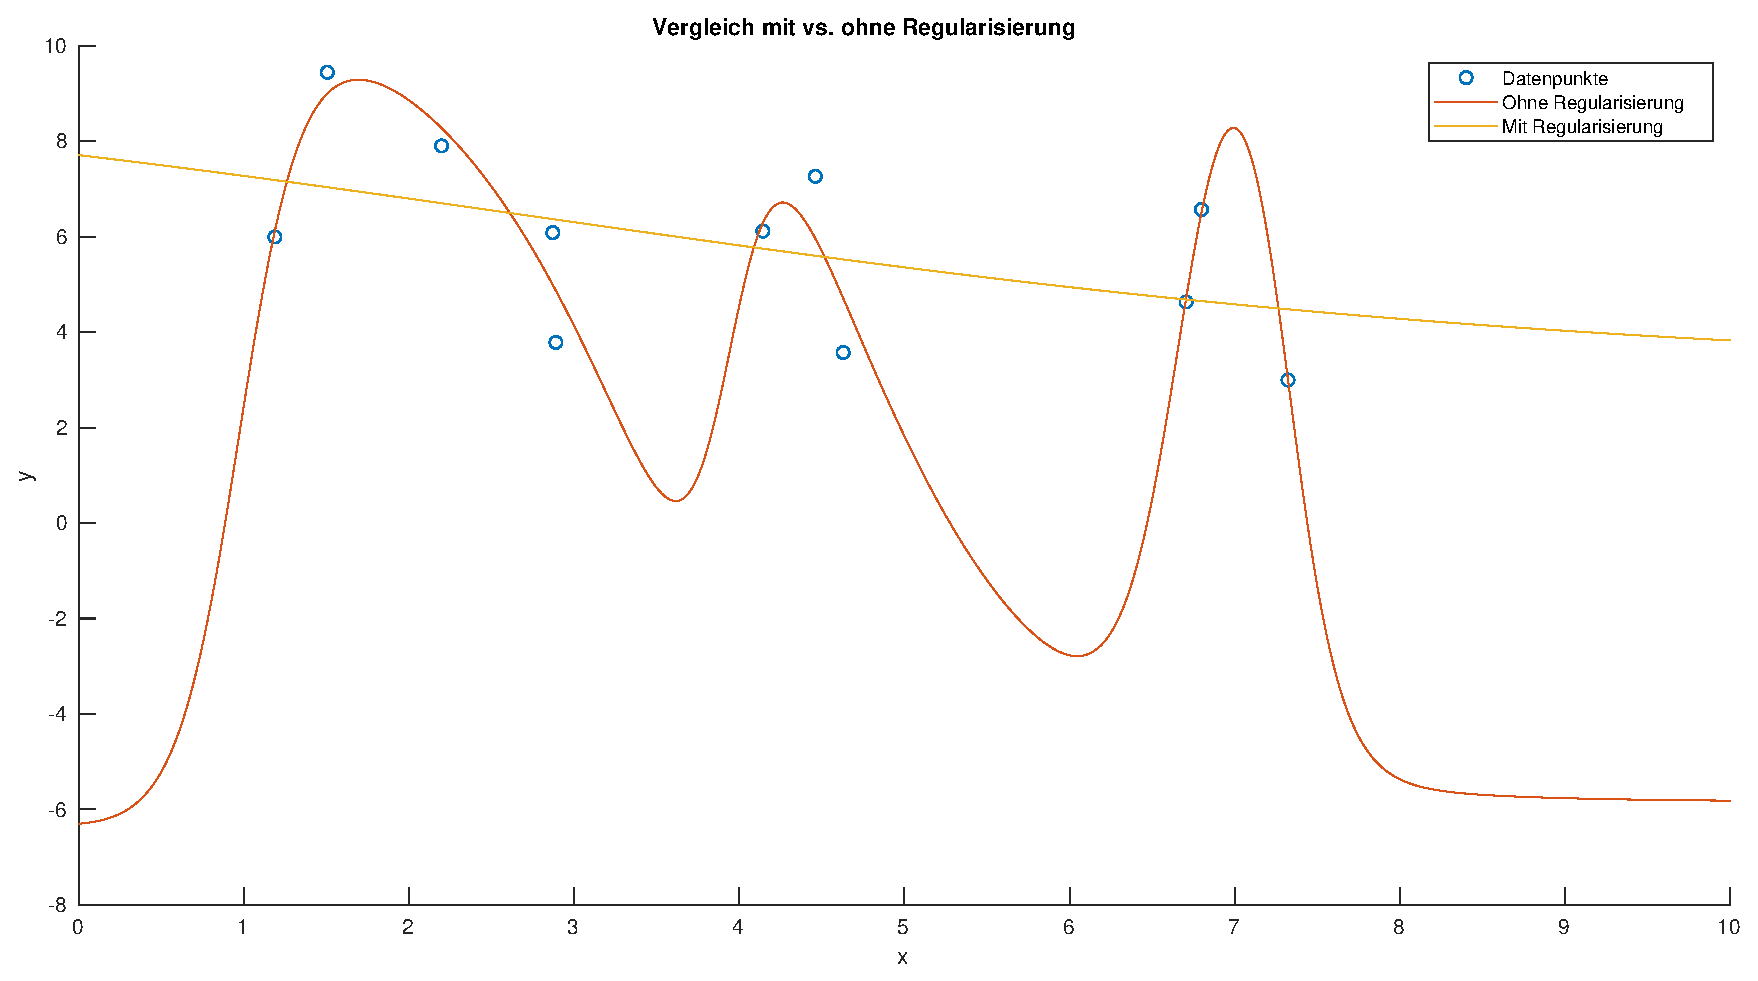
\includegraphics[width=\textwidth]{b08a02.eps}
            \end{figure}
    \end{enumerate}
\end{document}
